\chapter{Statistics of Chemical Measurement}\label{ch:b2:measurement-statistics}

Two laboratories measure the lead in the same tap water and report 9.6 and \qty{11.2}{\micro g/L}.
The guideline value for drinking water is \qty{10}{\micro g/L}. Is the water fit to drink? Do the two
laboratories even disagree, or are both results the same value seen through the scatter of two
measurements? A number from an analysis means nothing without its uncertainty, and this chapter gives
the tools to compute it: the statistics of repeated measurements, the propagation of uncertainties
through a calculation, calibration by least squares, and the limits below which a method sees nothing.
% ledger: who:lead

\begin{omfigure}
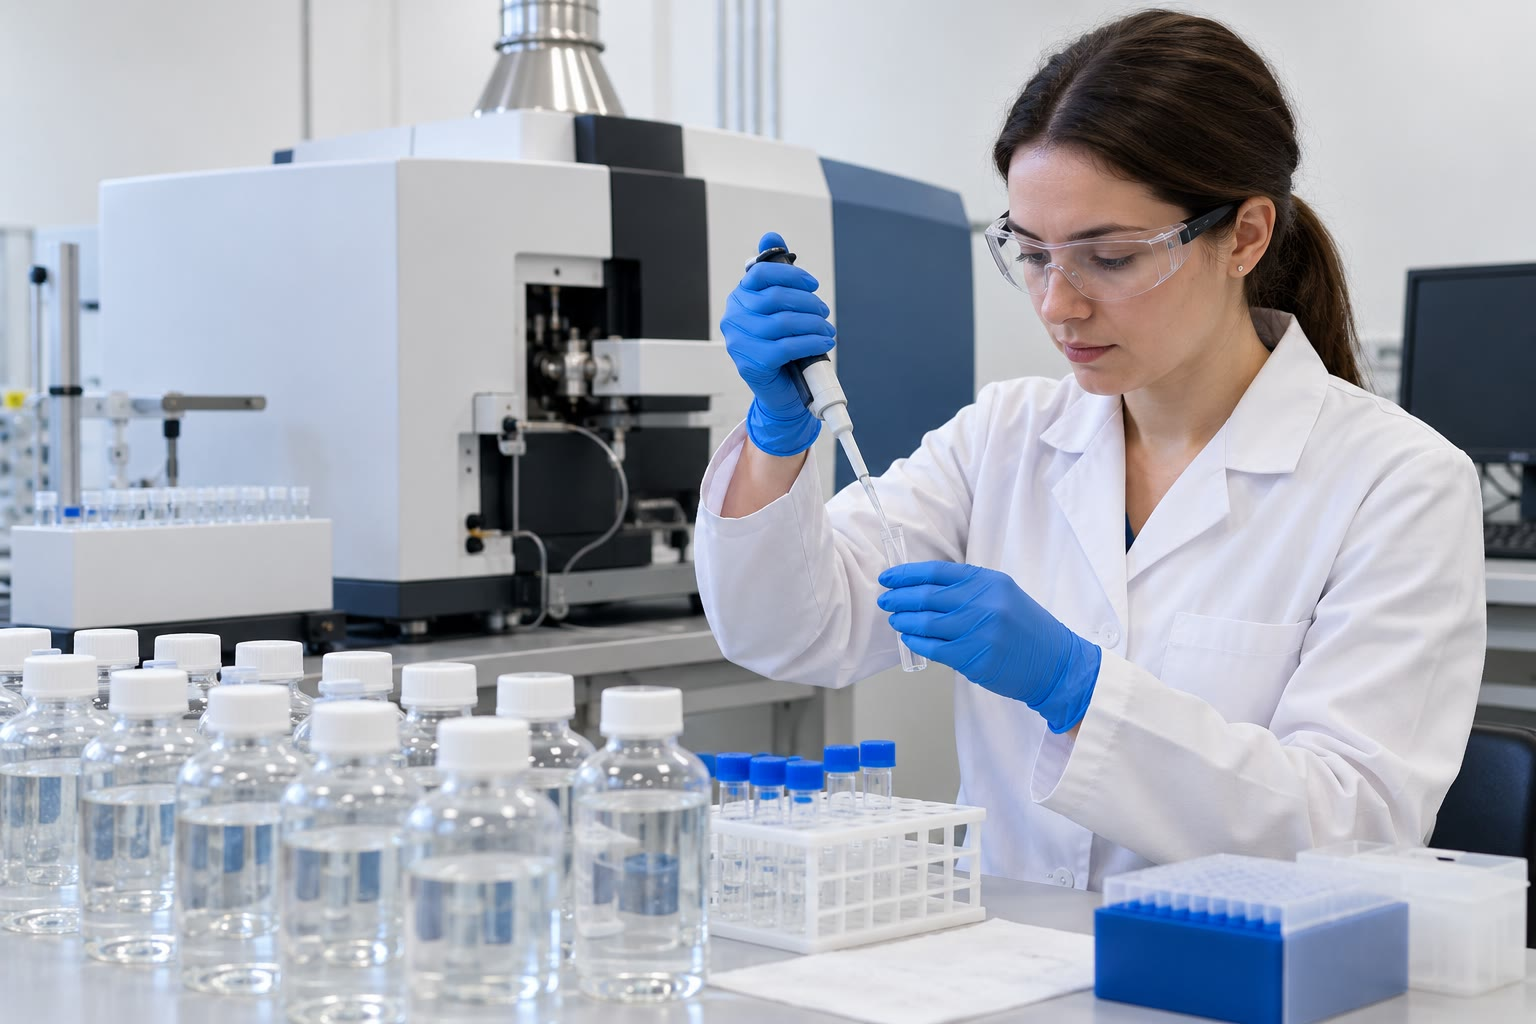
\includegraphics[width=0.56\linewidth]{images/book3/ai/b2-34-water-lab.jpg}

{\small A water-testing laboratory: sample bottles, a technician pipetting, an elemental analyser
behind (illustration).}
\end{omfigure}

\begin{recall}
The Year 1 volume: measurement uncertainty, standard uncertainty, type A and type B evaluations,
expanded uncertainty, relative uncertainty, the normalised deviation $z$ between two values, and the
promise of a proof of $u(\bar x) = s/\sqrt n$ and of a general propagation rule. The school volume: the
calibration line. \Cref{ch:b2:mass-spec-atomic}: atomic absorption.
\end{recall}

\section{Repeated measurements}

Repeat a measurement and the results scatter. We treat each result $x_i$ as a random variable with
mean $\mu$ (the value the method would give on average) and standard deviation $\sigma$; when many
small independent causes add up, the results follow the normal (Gaussian) law, about 68~\% of them
within $\mu \pm \sigma$ and 95~\% within $\mu \pm 1.96\sigma$.

\begin{definition}[Dispersion]\label{def:b2:measurement-statistics:dispersion}
For $n$ results $x_1, \dots, x_n$ of mean $\bar x$, the \emph{experimental standard
deviation}\index{experimental standard deviation} is $s = \sqrt{\sum (x_i - \bar x)^2/(n-1)}$; it
estimates $\sigma$. The \emph{standard deviation of the mean}\index{standard deviation of the mean} is
the standard deviation of $\bar x$ over many series of $n$ results, estimated by $s/\sqrt n$.
\end{definition}

The divisor $n - 1$ rather than $n$ corrects for the fact that the deviations are taken from $\bar x$,
itself computed from the same data, which makes them slightly too small: $n - 1$ is the number of
independent deviations, the degrees of freedom.

\begin{theorem}[Variance of the mean]\label{thm:b2:measurement-statistics:mean-variance}
If $x_1, \dots, x_n$ are independent, each of variance $\sigma^2$, then $\operatorname{var}(\bar x) =
\sigma^2/n$: the \omterm{def:b2:measurement-statistics:dispersion}{standard deviation of the mean} is $\sigma/\sqrt n$.
\end{theorem}

\begin{proof}
For independent variables the variance of a sum is the sum of the variances, and
$\operatorname{var}(cX) = c^2\operatorname{var}(X)$. So $\operatorname{var}(\bar x) =
\operatorname{var}\bigl(\tfrac1n\sum x_i\bigr) = \tfrac{1}{n^2}\sum\operatorname{var}(x_i) =
\tfrac{1}{n^2}\,n\sigma^2 = \sigma^2/n$. Replacing $\sigma$ by its estimate $s$ gives the type A
standard uncertainty $u(\bar x) = s/\sqrt n$ admitted in the Year 1 volume.
\end{proof}

\section{Confidence intervals}

\begin{definition}[Confidence interval]\label{def:b2:measurement-statistics:confidence}
A \emph{confidence interval}\index{confidence interval} at \emph{confidence level}\index{confidence level}
$1 - \alpha$ (often 95~\%) is an interval computed from the data by a rule that, applied to
many series, contains the true value in a fraction $1 - \alpha$ of them. For the mean of $n$ results it
is $\bar x \pm t\,s/\sqrt n$, where $t$ is \emph{Student's coefficient}\index{Student's coefficient}
for $n - 1$ degrees of freedom and that level.
\end{definition}

\begin{proposition}[Student's law]\label{prop:b2:measurement-statistics:student}
For $n$ independent normal results, $T = (\bar x - \mu)/(s/\sqrt n)$ follows Student's law with
$n - 1$ degrees of freedom, whose density is proportional to $(1 + t^2/\nu)^{-(\nu+1)/2}$ with
$\nu = n - 1$. It is wider than the normal law and tends to it as $n$ grows.
\end{proposition}

\admitted

Dividing by $s$ instead of the unknown $\sigma$ adds the scatter of $s$ itself, which is large when $n$ is
small; hence the heavier tails, and coefficients larger than 1.96. The table gives the 95~\%
coefficients, computed from the density.

\begin{omfigure}
\begin{minipage}[c]{0.56\linewidth}
\begin{tikzpicture}
\begin{axis}[width=\linewidth, height=4.8cm, xmin=-5, xmax=5, ymin=0, ymax=0.43,
  xlabel={$t$}, ylabel={density}, label style={font=\small}, tick label style={font=\scriptsize},
  legend style={font=\scriptsize, at={(0.98,0.98)}, anchor=north east}, legend cell align=left]
\addplot[omThm, thick] table[x=t, y=nu2] {figdata/out/bachelor-2-regression-c.dat};
\addplot[omMeth, thick] table[x=t, y=nu5] {figdata/out/bachelor-2-regression-c.dat};
\addplot[black, thick, dashed] table[x=t, y=normal] {figdata/out/bachelor-2-regression-c.dat};
\legend{$\nu = 2$, $\nu = 5$, normal}
\end{axis}
\end{tikzpicture}
\end{minipage}\hfill
\begin{minipage}[c]{0.4\linewidth}\centering
\small
\begin{tabular}{rr}
\hline
$\nu = n - 1$ & $t$ (95~\%) \\
\hline
1 & 12.706 \\
2 & 4.303 \\
3 & 3.182 \\
4 & 2.776 \\
5 & 2.571 \\
9 & 2.262 \\
20 & 2.086 \\
$\infty$ & 1.960 \\
\hline
\end{tabular}
\end{minipage}
\par\vspace{4pt}

{\small Student densities for 2 and 5 degrees of freedom against the normal law, and the two-sided
95~\% coefficients, computed by integrating the density (the last line is the normal law).}
% figdata: bachelor-2/regression.py parts c, e
\end{omfigure}

\begin{method}[A confidence interval for a mean]\label{met:b2:measurement-statistics:confidence-interval}
\begin{enumerate}
  \item Compute $\bar x$ and $s$ of the $n$ results; check that no result is grossly out of line.
  \item Read $t$ for $\nu = n - 1$ at the chosen level.
  \item Report $\bar x \pm t\,s/\sqrt n$, with the uncertainty rounded to one or two significant digits
        and the mean to the same decimal place.
  \item To compare with a reference value $x_{\mathrm{ref}}$, compute $|\bar x - x_{\mathrm{ref}}|/(s/\sqrt
        n)$: above $t$, the difference is significant at that level; below, the data do not show a
        difference (which does not prove there is none).
\end{enumerate}
\end{method}

\section{Propagation of uncertainty}

\begin{theorem}[Law of propagation of uncertainty]\label{thm:b2:measurement-statistics:propagation}
If $y = f(x_1, \dots, x_n)$, where the $x_i$ are independent with standard uncertainties $u(x_i)$ small
enough for $f$ to be nearly linear over them, then
\begin{equation*}
u^2(y) = \sum_{i=1}^{n}\left(\frac{\partial f}{\partial x_i}\right)^2 u^2(x_i).
\end{equation*}
\end{theorem}

\begin{proof}
To first order (Taylor), $y - f(\mu_1, \dots, \mu_n) \approx \sum c_i(x_i - \mu_i)$ with $c_i = \partial
f/\partial x_i$ at the means. The variance of a linear combination of independent variables is
$\sum c_i^2\operatorname{var}(x_i)$ (as in \cref{thm:b2:measurement-statistics:mean-variance}); with
$\operatorname{var}(x_i) = u^2(x_i)$ this is the result.
\end{proof}

\begin{corollary}[Sums and products]\label{cor:b2:measurement-statistics:products}
For a sum or difference, the standard uncertainties add in quadrature: $u^2(x_1 \pm x_2) = u^2(x_1) +
u^2(x_2)$. For a product or quotient $y = x_1^{a}x_2^{b}\cdots$, the relative uncertainties add in
quadrature, each weighted by its exponent: $\bigl(u(y)/y\bigr)^2 = a^2\bigl(u(x_1)/x_1\bigr)^2 +
b^2\bigl(u(x_2)/x_2\bigr)^2 + \cdots$
\end{corollary}

\begin{proof}
For a sum the partial derivatives are $\pm1$. For $y = x_1^ax_2^b$, $\partial y/\partial x_1 =
a\,y/x_1$ and $\partial y/\partial x_2 = b\,y/x_2$; the theorem gives $u^2(y) = a^2y^2u^2(x_1)/x_1^2 +
b^2y^2u^2(x_2)/x_2^2$; divide by $y^2$.
\end{proof}

\begin{method}[Propagating]\label{met:b2:measurement-statistics:propagate}
\begin{enumerate}
  \item Write the result as a formula of the measured quantities; list each input with its standard
        uncertainty (type A or B).
  \item For products and quotients, work with relative uncertainties; for sums, with absolute ones;
        otherwise take partial derivatives.
  \item Combine in quadrature; find the dominant term: improving the others is wasted effort.
  \item Multiply by the coverage factor (2, or Student's $t$ when the dominant term comes from few
        repeats) for an expanded uncertainty.
\end{enumerate}
\end{method}

\section{Calibration}

\begin{definition}[Calibration curve]\label{def:b2:measurement-statistics:calibration}
A \emph{calibration curve}\index{calibration curve} relates the signal $y$ of an instrument to the
concentration $x$, from standards of known concentration. The \emph{least-squares
line}\index{least-squares line} $y = a + bx$ is the line that minimises $S = \sum (y_i - a -
bx_i)^2$; each $e_i = y_i - a - bx_i$ is a \emph{residual}\index{residual}.
\end{definition}

\begin{theorem}[Least-squares line]\label{thm:b2:measurement-statistics:least-squares}
With $\bar x$, $\bar y$ the means, $S_{xx} = \sum(x_i - \bar x)^2$ and $S_{xy} = \sum(x_i - \bar x)(y_i -
\bar y)$, the \omterm{def:b2:measurement-statistics:calibration}{least-squares line} has
\begin{equation*}
b = \frac{S_{xy}}{S_{xx}}, \qquad a = \bar y - b\bar x.
\end{equation*}
\end{theorem}

\begin{proof}
$S$ is a quadratic function of $a$ and $b$. Its partial derivatives vanish at the minimum:
$\partial S/\partial a = -2\sum(y_i - a - bx_i) = 0$ gives $a = \bar y - b\bar x$; substituting in
$\partial S/\partial b = -2\sum x_i(y_i - a - bx_i) = 0$ gives $\sum x_i\bigl((y_i - \bar y) - b(x_i -
\bar x)\bigr) = 0$, that is $S_{xy} = bS_{xx}$ (since $\sum \bar x(y_i - \bar y) = \sum \bar x(x_i - \bar
x) = 0$). The second derivatives form the matrix
\[\begin{pmatrix} 2n & 2\sum x_i\\ 2\sum x_i & 2\sum x_i^2\end{pmatrix},\]
whose diagonal is positive and whose determinant $4nS_{xx}$ is positive when the $x_i$ are not all
equal: the stationary point is a minimum.
\end{proof}

\begin{proposition}[Reading a concentration]\label{prop:b2:measurement-statistics:interpolation}
For $n$ standards with \omterm{def:b2:measurement-statistics:calibration}{residual} standard deviation $s_{y/x} = \sqrt{\sum e_i^2/(n-2)}$, a sample read
$m$ times with mean signal $\bar y_0$ has $x_0 = (\bar y_0 - a)/b$ and standard deviation
\begin{equation*}
s_{x_0} = \frac{s_{y/x}}{b}\sqrt{\frac1m + \frac1n + \frac{(\bar y_0 - \bar y)^2}{b^2S_{xx}}},
\end{equation*}
to be used with Student's $t$ for $n - 2$ degrees of freedom.
\end{proposition}

\admitted

The three terms under the root are the scatter of the sample readings, the uncertainty of the line's
height and that of its slope; the last vanishes at the centre of the calibration range, which is where
samples are best read.

\begin{omfigure}
\begin{tikzpicture}
\begin{axis}[width=0.5\linewidth, height=5cm, xmin=-1, xmax=22, ymin=0, ymax=0.22,
  xlabel={lead (\unit{\micro g/L})}, ylabel={absorbance}, label style={font=\small},
  tick label style={font=\scriptsize}, scaled y ticks=false,
  yticklabel style={/pgf/number format/fixed, /pgf/number format/precision=2}]
\addplot[omDef, thick] table[x=x, y=line] {figdata/out/bachelor-2-regression-b.dat};
\addplot[only marks, mark=*, mark size=1.8pt, omThm] table[x=x, y=A] {figdata/out/bachelor-2-regression-a.dat};
\end{axis}
\end{tikzpicture}\hfill
\begin{tikzpicture}
\begin{axis}[width=0.5\linewidth, height=5cm, xmin=-1, xmax=22, ymin=-0.002, ymax=0.002,
  xlabel={lead (\unit{\micro g/L})}, ylabel={residual}, label style={font=\small},
  tick label style={font=\scriptsize}, scaled y ticks=false, ycomb,
  yticklabel style={/pgf/number format/fixed, /pgf/number format/precision=3},
  extra y ticks={0}, extra y tick style={grid=major, grid style={black!50}}]
\addplot[omThm, thick, mark=*, mark size=1.6pt] table[x=x, y=res] {figdata/out/bachelor-2-regression-a.dat};
\end{axis}
\end{tikzpicture}

{\small Calibration of lead by graphite-furnace atomic absorption at \qty{283.3}{nm} (exercise data,
used in the problem). Left: the five standards and the \omterm{def:b2:measurement-statistics:calibration}{least-squares line}. Right: the \omterm{def:b2:measurement-statistics:calibration}{residuals}, small
and without pattern: a straight line is adequate.}
% figdata: bachelor-2/regression.py parts a, b
% ledger: asd:Pb283
\end{omfigure}

\begin{method}[Calibrating]\label{met:b2:measurement-statistics:calibrate}
\begin{enumerate}
  \item Prepare five or more standards spanning the expected range, in the same matrix as the samples,
        and a blank.
  \item Fit the \omterm{def:b2:measurement-statistics:calibration}{least-squares line}; plot the \omterm{def:b2:measurement-statistics:calibration}{residuals}. A curved pattern means the response is not
        linear: narrow the range or fit a curve. One large \omterm{def:b2:measurement-statistics:calibration}{residual} points to a faulty standard.
  \item Read the samples, preferably near the middle of the range, in replicate; compute $x_0$ and
        $s_{x_0}$.
  \item Report $x_0 \pm t\,s_{x_0}$ after correcting for every dilution, with the propagated uncertainty
        of the dilution added if it is not negligible.
\end{enumerate}
\end{method}

\begin{definition}[Standard addition]\label{def:b2:measurement-statistics:standard-addition}
In the \emph{standard-addition method}\index{standard-addition method}, known amounts of analyte are
added to equal portions of the sample itself; the signal is plotted against the concentration added,
and the concentration of the analyte in the sample is the distance from the origin to the point where
the line extrapolated to zero signal crosses the axis, $a/b$.
\end{definition}

\begin{method}[Standard addition]\label{met:b2:measurement-statistics:standard-addition}
\begin{enumerate}
  \item Use it when the sample matrix changes the response (salts, acids, organic matter), so that
        standards in pure water would give a wrong slope.
  \item Spike equal portions with increasing known amounts, dilute all to the same volume, measure.
  \item Fit the line; the concentration in the measured solutions is $a/b$; correct for the dilution.
  \item The response must be linear from zero: check the \omterm{def:b2:measurement-statistics:calibration}{residuals}.
\end{enumerate}
\end{method}

\begin{omfigure}
\begin{tikzpicture}
\begin{axis}[width=0.62\linewidth, height=5cm, xmin=-4, xmax=7, ymin=0, ymax=0.42,
  xlabel={concentration added (\unit{mg/L})}, ylabel={absorbance}, label style={font=\small},
  tick label style={font=\scriptsize}, axis lines=left, scaled y ticks=false,
  yticklabel style={/pgf/number format/fixed, /pgf/number format/precision=1}]
\draw[black!40] (axis cs:0,0) -- (axis cs:0,0.42);
\addplot[omDef, thick, densely dashed] table[x=x, y=line] {figdata/out/bachelor-2-regression-d-line.dat};
\addplot[only marks, mark=*, mark size=1.8pt, omThm] table[x=x, y=A] {figdata/out/bachelor-2-regression-d.dat};
\draw[<->, omMeth, thick] (axis cs:-3.11,0.06) -- (axis cs:0,0.06); \node[omMeth, below, font=\scriptsize] at (axis cs:-0.8,0.055) {$a/b$};
\end{axis}
\end{tikzpicture}

{\small Standard addition (exercise data): absorbance of a sample spiked with 0, 2, 4 and
\qty{6}{mg/L} of analyte. The line meets zero signal at \qty{-3.11}{mg/L}: the measured solution
contained \qty{3.11}{mg/L}.}
% figdata: bachelor-2/regression.py part d
\end{omfigure}

\section{Detection, quantification and validation}

\begin{definition}[Limits]\label{def:b2:measurement-statistics:limits}
The \emph{limit of detection}\index{limit of detection} of a method is the smallest concentration whose
signal can be distinguished from that of a blank with a stated small risk of a false detection; the
\emph{limit of quantification}\index{limit of quantification} is the smallest concentration that can
be measured with an acceptable relative uncertainty.
\end{definition}

\begin{proposition}[Common estimates]\label{prop:b2:measurement-statistics:lod}
With $s_{\mathrm{blank}}$ the standard deviation of repeated blank signals and $b$ the slope of the
calibration line, $x_{\mathrm{LOD}} \approx 3s_{\mathrm{blank}}/b$ and $x_{\mathrm{LOQ}} \approx
10s_{\mathrm{blank}}/b$.
\end{proposition}

\begin{proof}[Argument]
If blank signals are normal with standard deviation $s_{\mathrm{blank}}$, a blank exceeds its mean by
more than $3s_{\mathrm{blank}}$ with probability about 0.13~\% (one-sided tail of the normal law beyond
3 standard deviations): calling a signal ``detected'' above that threshold rarely mistakes a blank for
a sample. A signal $10s_{\mathrm{blank}}$ above the blank has a relative standard deviation of about
10~\%, the usual threshold for a quantitative result. Dividing by $b$ converts signals into
concentrations.
\end{proof}

\begin{definition}[Validation]\label{def:b2:measurement-statistics:validation}
\emph{Trueness}\index{trueness} is the closeness of the mean of a large number of results to the true
value; their difference is the \emph{bias}\index{bias}. \emph{Precision}\index{precision} is the
closeness of independent results to each other, expressed as a standard deviation:
\emph{repeatability}\index{repeatability} under the same conditions (same operator, instrument,
laboratory, short time), \emph{reproducibility}\index{reproducibility} under changed conditions
(different laboratories). \emph{Method validation}\index{method validation} is the set of experiments
that establish, for a method, its trueness, precision, linearity and range, and its limits of detection
and quantification.
\end{definition}

\omterm{def:b2:measurement-statistics:validation}{Trueness} is checked against a certified reference material or by spiking; \omterm{def:b2:measurement-statistics:validation}{precision} by replicates in
one laboratory and by comparisons between laboratories. A method can be precise but biased, every
result close to the others and all of them wrong: \omterm{def:b2:measurement-statistics:validation}{precision} is no proof of \omterm{def:b2:measurement-statistics:validation}{trueness}.

\begin{history}[Student, 1908]
\begin{minipage}[t]{0.17\linewidth}
\vspace{0pt}
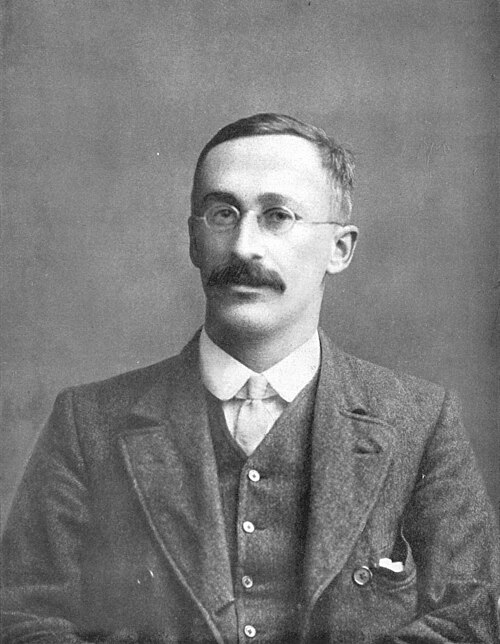
\includegraphics[width=\linewidth]{images/book3/gosset.jpg}
\end{minipage}\hfill
\begin{minipage}[t]{0.79\linewidth}
\vspace{0pt}
William Sealy Gosset, a chemist working for a brewery, had to judge raw materials from very few samples,
far too few for the normal law. In 1908 he published the distribution of the mean divided by the sample
standard deviation, under the pen name ``Student'' because his employer did not allow staff to publish
under their names. Student's law is used every time an analyst quotes an interval from three or four
replicates. (Photograph, 1908: public domain; Wikimedia Commons.)
\end{minipage}
\end{history}

\section{Exercises}

\begin{exercise}[$\star$]\label{exo:b2:measurement-statistics:1}
Five titrations give 12.45, 12.50, 12.48, 12.52 and \qty{12.46}{mL}. Compute the mean, the
\omterm{def:b2:measurement-statistics:dispersion}{experimental standard deviation} and the \omterm{def:b2:measurement-statistics:dispersion}{standard deviation of the mean}.
\end{exercise}

\begin{exercise}[$\star$]\label{exo:b2:measurement-statistics:2}
Give the 95~\% \omterm{def:b2:measurement-statistics:confidence}{confidence interval} of the mean of exercise~1.
\end{exercise}

\begin{exercise}[$\star$]\label{exo:b2:measurement-statistics:3}
A solution is made by dissolving $m = \qty{0.5000}{g}$ ($u = \qty{0.0002}{g}$) of a solid in a flask of
$V = \qty{250.0}{mL}$ ($u = \qty{0.15}{mL}$). Compute the relative standard uncertainty of $c = m/(MV)$,
the molar mass being exact enough.
\end{exercise}

\begin{exercise}[$\star$]\label{exo:b2:measurement-statistics:4}
Fit the \omterm{def:b2:measurement-statistics:calibration}{least-squares line} through $(0, 0.02)$, $(1, 0.21)$, $(2, 0.39)$, $(3, 0.62)$.
\end{exercise}

\begin{exercise}[$\star\star$]\label{exo:b2:measurement-statistics:5}
A certified reference solution contains \qty{10.00}{mg/L} of an element. Five analyses give a mean of
\qty{10.12}{mg/L} with $s = \qty{0.08}{mg/L}$. Is the method biased at the 95~\% level?
\end{exercise}

\begin{exercise}[$\star\star$]\label{exo:b2:measurement-statistics:6}
A concentration of hydronium ions is known with a relative standard uncertainty of 2~\%. What is the
standard uncertainty of the pH?
\end{exercise}

\begin{exercise}[$\star\star$]\label{exo:b2:measurement-statistics:7}
Ten blanks have $s = 0.0012$ absorbance units; the calibration slope is \qty{0.0098}{L/\micro g}.
Estimate the limits of detection and of quantification.
\end{exercise}

\begin{exercise}[$\star\star$]\label{exo:b2:measurement-statistics:8}
In the standard-addition experiment of the figure, the four portions had been made by diluting
\qty{10.0}{mL} of sample to \qty{50.0}{mL}. Give the concentration in the sample.
\end{exercise}

\begin{exercise}[$\star\star$]\label{exo:b2:measurement-statistics:9}
In an interlaboratory study, each laboratory obtains $s = \qty{0.05}{mg/L}$ on its own replicates, but
the results of different laboratories scatter with $s = \qty{0.15}{mg/L}$. Name the two quantities and
explain the difference.
\end{exercise}

\begin{exercise}[$\star\star\star$]\label{exo:b2:measurement-statistics:10}
Show that the \omterm{def:b2:measurement-statistics:calibration}{least-squares line} passes through $(\bar x, \bar y)$ and that its \omterm{def:b2:measurement-statistics:calibration}{residuals} sum to zero.
\end{exercise}

\begin{exercise}[$\star\star\star$]\label{exo:b2:measurement-statistics:11}
A stock solution is diluted a hundredfold either in one step (\qty{1.000}{mL} into \qty{100.0}{mL}) or
in two tenfold steps (\qty{10.00}{mL} into \qty{100.0}{mL}, twice). Standard uncertainties: 1 mL
pipette \qty{0.006}{mL}, 10 mL pipette \qty{0.02}{mL}, 100 mL flask \qty{0.08}{mL} (exercise data).
Which route is more precise?
\end{exercise}

\begin{exercise}[$\star\star\star$]\label{exo:b2:measurement-statistics:12}
The two laboratories of the opening report 9.6 and \qty{11.2}{\micro g/L} with standard uncertainties
0.4 and \qty{0.5}{\micro g/L} (exercise data). Are their results compatible? What does each say about the
guideline value?
\end{exercise}

\section{Problem: Lead in Tap Water}

\begin{problem}[{Weekend problem --- an atomic-absorption calibration by least squares, the
concentration of a sample with its confidence interval, the dilution and the limits, and a verdict
against the guideline value}]
\label{pb:b2:measurement-statistics:1}
Exercise data. Lead is measured by graphite-furnace atomic absorption at \qty{283.3}{nm}. Standards
(\unit{\micro g/L}; absorbance): 0.0; 0.003, 5.0; 0.051, 10.0; 0.101, 15.0; 0.148, 20.0; 0.199. The
tap water (\qty{50.0}{mL}) is acidified with \qty{0.50}{mL} of nitric acid; three readings of this
solution give 0.104, 0.098 and 0.101. Ten blanks: 0.002, 0.004, 0.003, 0.001, 0.003, 0.005, 0.002,
0.003, 0.004, 0.003. Standard uncertainties of the volumes: \qty{0.03}{mL} for 50.0 mL,
\qty{0.005}{mL} for 0.50 mL. Guideline value: \qty{10}{\micro g/L}.
% ledger: who:lead, asd:Pb283

\medskip
\noindent\textbf{Part I --- Calibration.}
\begin{enumerate}
  \item Why are the standards prepared in the same nitric acid as the samples?
  \item Compute the slope and the intercept of the \omterm{def:b2:measurement-statistics:calibration}{least-squares line}.
  \item Compute the five \omterm{def:b2:measurement-statistics:calibration}{residuals}.
  \item Do the \omterm{def:b2:measurement-statistics:calibration}{residuals} show a pattern? Conclude on linearity.
  \item Compute $s_{y/x}$.
  \item Why is the intercept not zero?
  \item What does the slope measure?
\end{enumerate}

\medskip
\noindent\textbf{Part II --- The sample.}
\begin{enumerate}[resume]
  \item Compute the mean and the standard deviation of the three readings.
  \item Compute the lead concentration of the measured solution.
  \item Compute $s_{x_0}$.
  \item How many degrees of freedom, and which Student coefficient?
  \item Give the 95~\% interval of the concentration in the measured solution.
  \item Why read the sample three times rather than once?
\end{enumerate}

\medskip
\noindent\textbf{Part III --- Dilution and limits.}
\begin{enumerate}[resume]
  \item Compute the dilution factor and the concentration in the tap water.
  \item Propagate the uncertainty of the two volumes into the dilution factor.
  \item Is that uncertainty significant beside the calibration one?
  \item Compute the standard deviation of the blanks and the \omterm{def:b2:measurement-statistics:limits}{limit of detection}.
  \item Compute the \omterm{def:b2:measurement-statistics:limits}{limit of quantification}.
  \item Is the sample above the \omterm{def:b2:measurement-statistics:limits}{limit of quantification}?
\end{enumerate}

\medskip
\noindent\textbf{Part IV --- Verdict.}
\begin{enumerate}[resume]
  \item Does the interval contain the guideline value?
  \item What would a single reading of 0.104 have suggested?
  \item What does ``95~\% confidence'' mean here?
  \item How could the laboratory decide more firmly?
  \item How would it check that the method is not biased?
  \item The guideline is provisional ``on the basis of treatment performance and analytical
        achievability''. What does the second reason mean, in the light of this problem?
  \item State the lead concentration of the tap water with its 95~\% interval, and compare it with
        \qty{10}{\micro g/L}.
\end{enumerate}
\end{problem}
